\documentclass[12pt]{beamer}
\usetheme{Warsaw}
\usepackage[utf8]{inputenc}
\usepackage{amsmath}
\usepackage{amsfonts}
\usepackage{amssymb}
\usepackage{graphicx}
\usepackage[font=Times,timeinterval=1,timeduration=2.0,timedeath=0,fillcolorwarningsecond=white!60!yellow,timewarningfirst=50,timewarningsecond=80,resetatpages=2]{tdclock}
\usepackage{tabularx}
\usepackage{array}
\usepackage{multicol}
\usepackage{longtable}
\usepackage{xcolor}
\usepackage{textcomp, gensymb}
\usepackage{pgfplots}
\usepackage[makeroom]{cancel}

\graphicspath{ {./references/} }
\pgfplotsset{
	soldot/.style={color=black,only marks,mark=*},
	holdot/.style={color=black,fill=white,only marks,mark=*},
	compat=1.12
}
\newcolumntype{Y}{>{\centering\arraybackslash}X}
\makeatletter
\def\@listii{\leftmargin\leftmarginii
			  \topsep    2ex
			  \parsep    0\p@   \@plus\p@
			  \itemsep   \parsep}
\makeatother
\newcommand\at[2]{\left.#1\right|_{#2}}

\begin{document}
\begin{frame}
	\frametitle{Bellwork 1/10}
	\initclock

	\begin{center}
		\large
		\underline{Graph of $f$}
		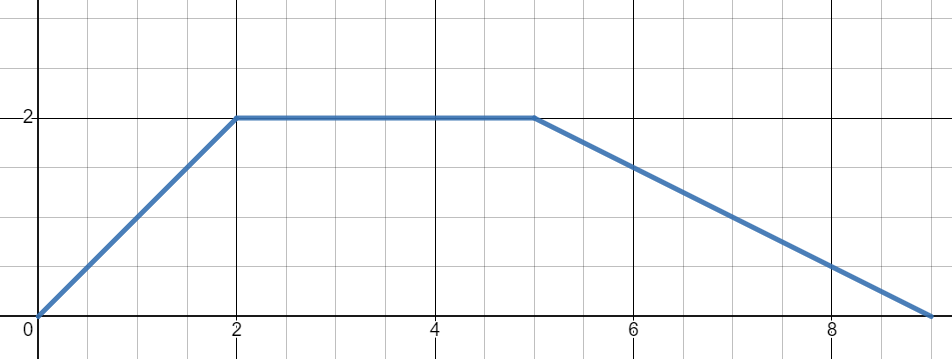
\includegraphics[scale=0.4]{bellwork_graph.png}\\
		Let $g(x) = \int_{5}^{x}f(s)ds$. Evaluate the following:
	\end{center}
	\[g(0)\text{, }g(2)\text{, }g(9)\]

	\vfill

	\small
	\crono
	\resetcrono{\beamerbutton{reset}}
\end{frame}
\begin{frame}
	\frametitle{Exercise 1}

	\vfill
	\vfill
	\Large
	\[f(x)=\int_{-5}^{x}edt\]
	\vfill
	\begin{center}
		Find $f(5)$ using part 2 of the FTC.
	\end{center}
	\vfill
	\vfill
\end{frame}
\begin{frame}
	\frametitle{Exercise 1 - Solution}

	\Large
	\begin{align*}
		f(5)=\int_{-5}^{5}edt
	\end{align*}
	\small
	\hrule
	\vfill
	\vfill
	The antiderivative of $\int edt$ is $et+C$ for some constant $C$.
	\large
	\begin{align*}
		\text{FTC 2}\implies \int_{-5}^{5}edt &= e(5)-e(-5) \\
		&= \boxed{10e}
	\end{align*}
	\vfill
	\vfill
	\vfill
\end{frame}
\begin{frame}
	\frametitle{Exercise 2}

	\vfill
	\vfill
	\Large
	\[g(x)=\int_{\frac{\pi}{4}}^{x}\csc^2\left(\theta\right)d\theta\]
	\vfill
	\begin{center}
		Find $g(\frac{\pi}{3})$ using part 2 of the FTC.
	\end{center}
	\vfill
	\vfill
\end{frame}
\begin{frame}
	\frametitle{Exercise 2 - Solution}

	\Large
	\begin{align*}
		g\left(\frac{\pi}{3}\right)=\int_{\frac{\pi}{4}}^{\frac{\pi}{3}}\csc^2\left(\theta\right)d\theta
	\end{align*}
	\small
	\hrule
	\vfill
	\vfill
	The antiderivative of $\int \csc^2\left(\theta\right)d\theta$ is $-\cot\left(\theta\right)+C$.
	\small
	\begin{align*}
		\text{FTC 2}\implies \int_{\frac{\pi}{4}}^{\frac{\pi}{3}}\csc^2\left(\theta\right)d\theta &= \left[-\cot\left(\frac{\pi}{3}\right)\right]-\left[-\cot\left(\frac{\pi}{4}\right)\right] \\
		&= \boxed{-\frac{\sqrt{3}}{3}+1}
	\end{align*}
	\vfill
	\vfill
	\vfill
\end{frame}
\begin{frame}
	\frametitle{Exercise 3}

	\vfill
	\vfill
	\Large
	\[h(x)=\int_{0}^{x}\left(2\sin{t}-e^t\right)dt\]
	\vfill
	\begin{center}
		Find $h(3)$ using part 2 of the FTC.
	\end{center}
	\vfill
	\vfill
\end{frame}
\begin{frame}
	\frametitle{Exercise 3 - Solution}

	\Large
	\begin{align*}
		h(3)=\int_{0}^{3}\left(2\sin{t}-e^t\right)dt
	\end{align*}
	\small
	\hrule
	\vfill
	\vfill
	The antiderivative of $\int \left(2\sin{t}-e^t\right)dt$ is $-2\cos(t)-e^t+C$.
	\small
	\begin{align*}
		\text{FTC 2}\implies \int_{0}^{3}\left(2\sin{t}-e^t\right)dt &= [-2\cos(3)-e^3]-[-2\cos(0)-e^0] \\
		&= \boxed{3-e^3-2\cos(3)}
	\end{align*}
	\vfill
	\vfill
	\vfill
\end{frame}
\end{document}